\section{Discussion: System Scope and Limitations}

\begin{figure*}[h!]
\centering
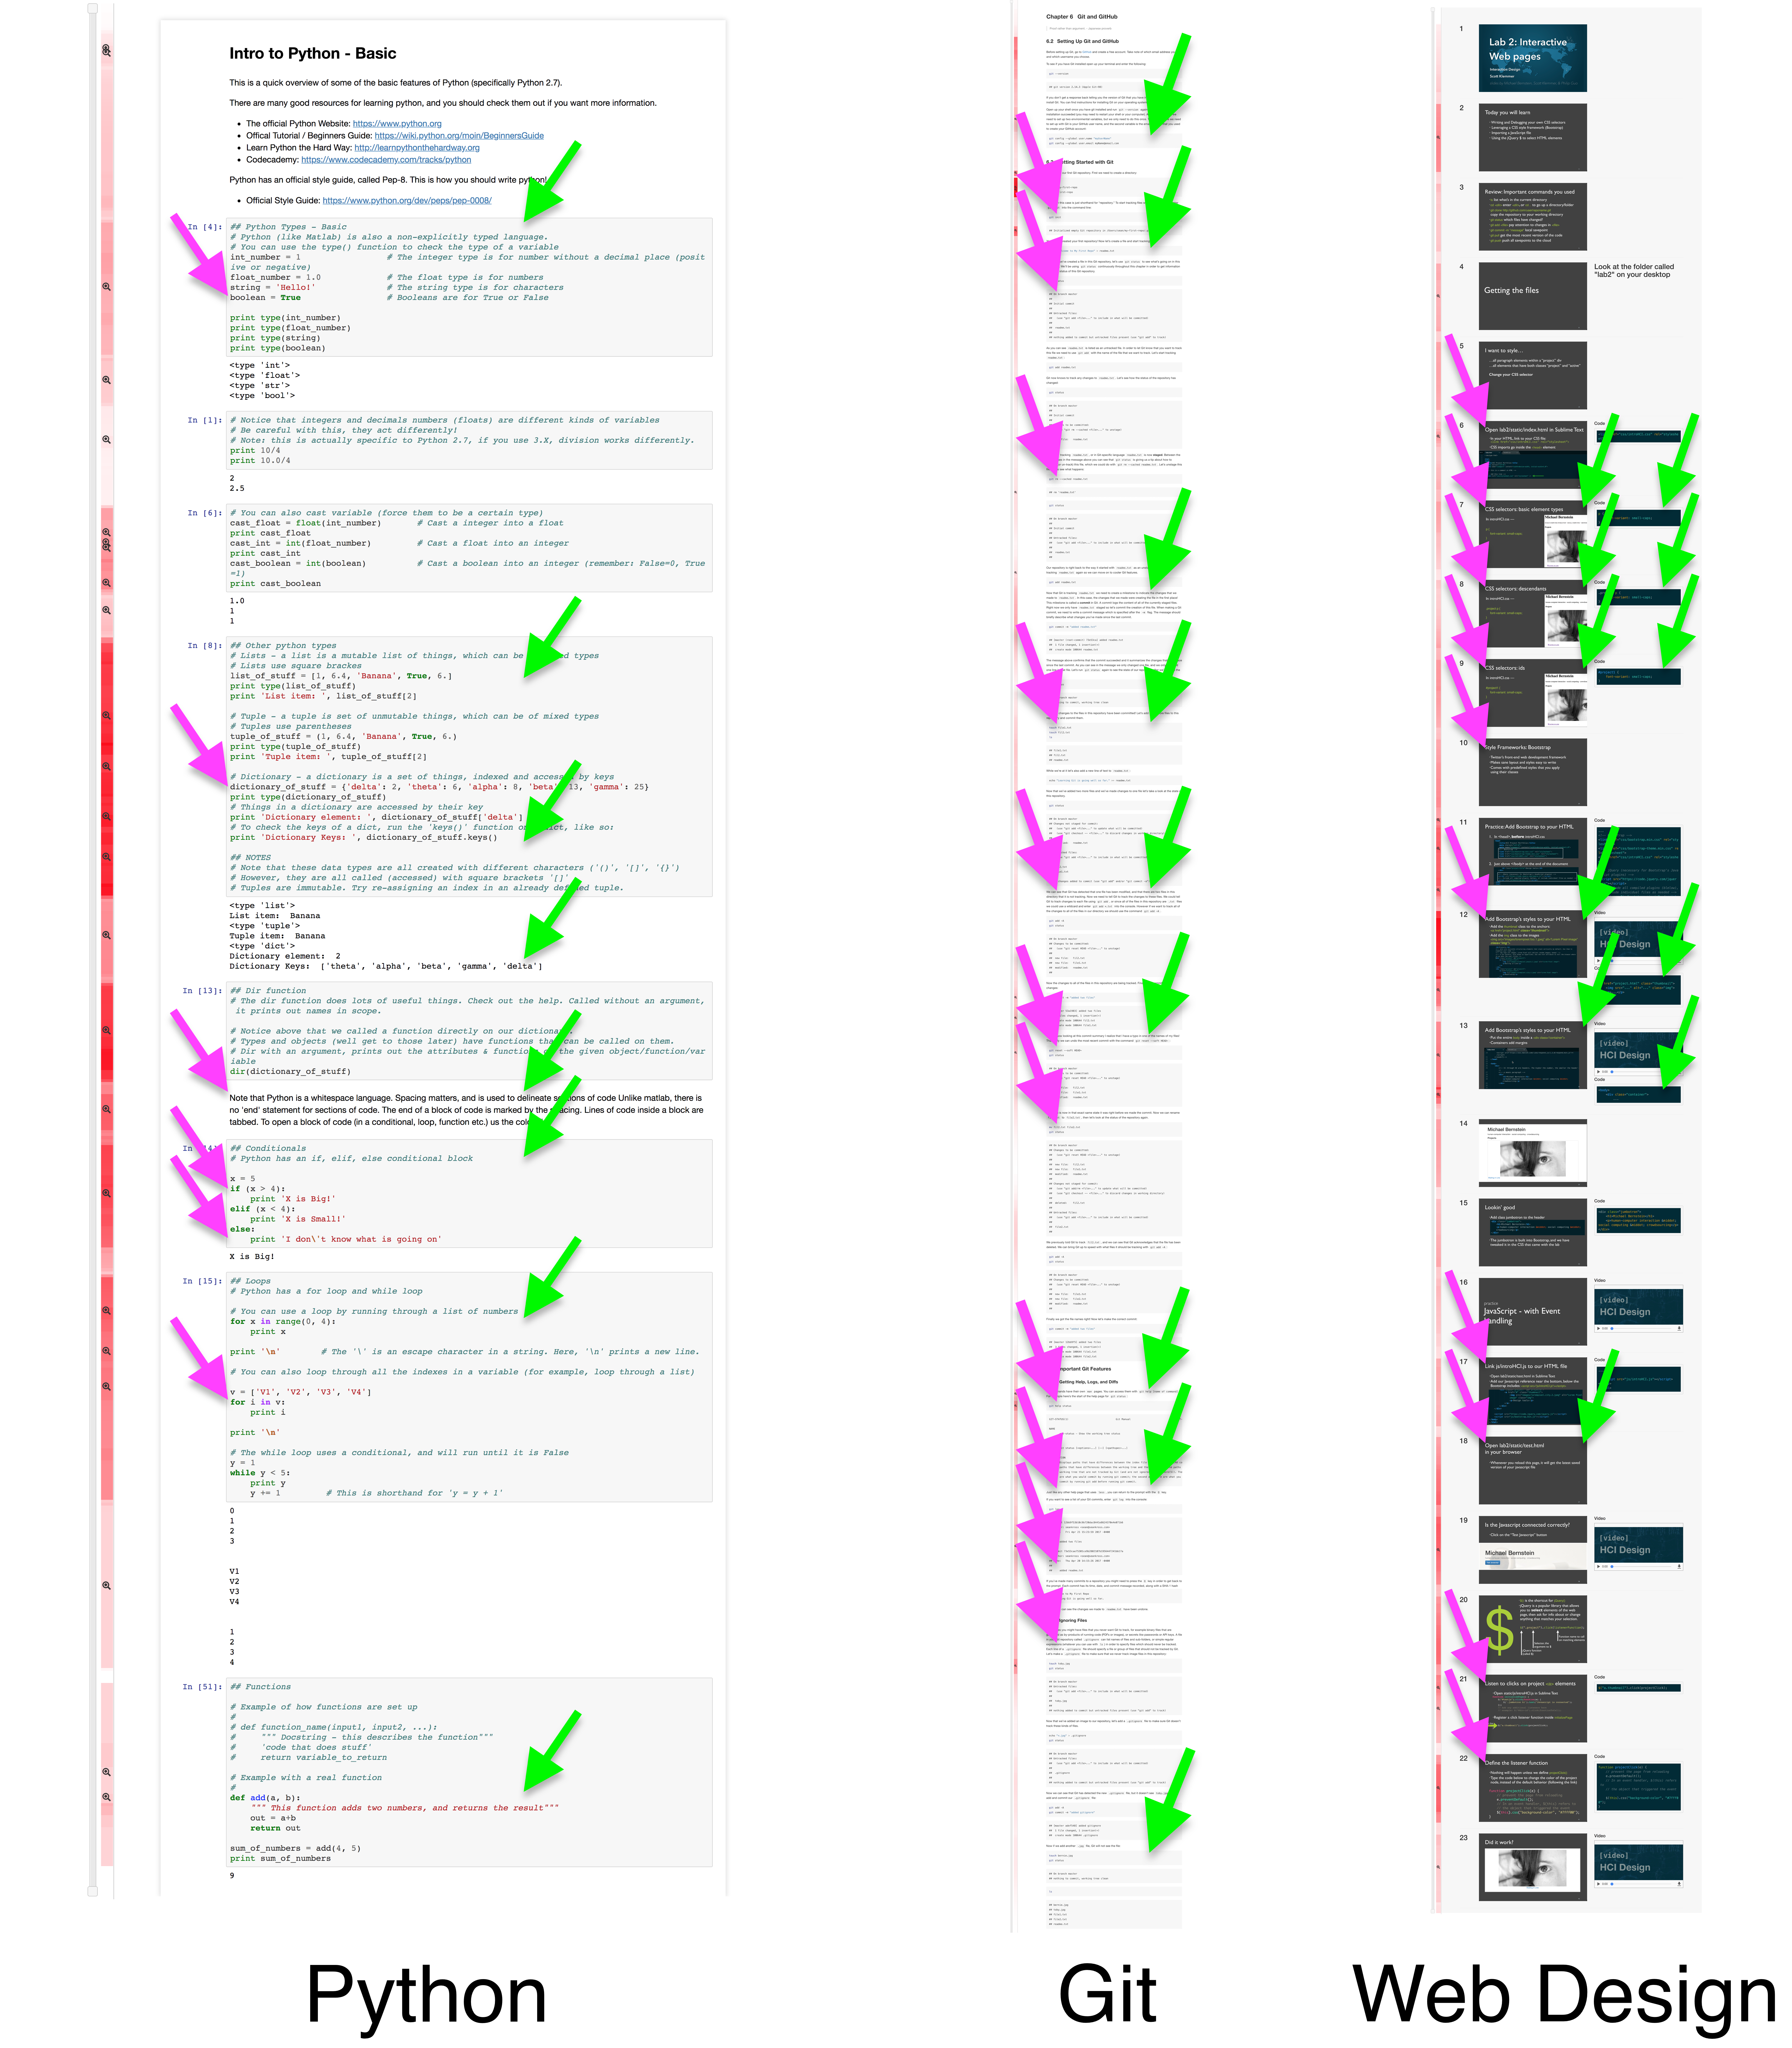
\includegraphics[width=1\columnwidth]{figures/porta/corrections.png}

\caption{Screenshots of all 3 tutorials with green arrows pointing to the improvements identified by the learners and pink arrows pointing to the improvements identified by the creators}

\vspace{-0.25em} % stent

\label{fig:corrections}
\end{figure*}

\fig{fig:corrections} gives an overview of all the improvements over all 3 tutorials by both the learners and creators.

Porta is best suited for profiling multi-application tutorials commonly
found in domains such as software engineering, web development, system
administration, and data science. It is less well-suited for detailed
profiling of single-application tutorials such as those for MS Word,
Excel, or Photoshop. Since Porta does not perform tracking within GUI
apps, the most it can do for those tutorials is display a general
heatmap and screencast videos.
%
One way to overcome this limitation is to build plug-ins that track
these applications in detail; then Porta can integrate their events into
its profiling visualization.

There is inherent imprecision to Porta's heatmaps since it is impossible
to tell where in the tutorial the participant is truly focusing on,
short of continually asking them. The Gaussian distribution is a crude
model for approximating uncertainty in positional focus. Time estimates
are also imprecise because Porta cannot easily tell whether the user is
on task, distracted, or taking a break.
%
%Though when used in a formal user test, there might be an implicit
%expectation to remain on task.
%
On a related note, is spending more time on a certain part of the
tutorial good or bad? Maybe it is good since that part is more engaging,
or maybe it is bad if there are lots of error-related events at those
parts. Thus, profile visualizations should be used \textbf{\emph{as a
substrate to facilitate discussion and reflection, not as a source of
precise ground truth}}.

Porta requires installing and running OS-wide monitoring software that
may lead to privacy concerns. When used in an in-person user test, it
can come pre-installed on the lab computer. The experimenter can brief
test participants on privacy implications and erase their test accounts
after each session. When used in online experiments, participants must
both be technically adept enough to install it and also put their trust
in it. To allay concerns about privacy leaks, participants can inspect
the raw data that Porta collects and view the profile visualizations,
which is exactly what the tutorial creator sees.
%
These logistical complexities mean that Porta is not well-suited for
longer-term always-on deployment in a field study. Rather, we envision it
being selectively activated only during user testing sessions, whether
in-person or remote.

Since Porta's positional heatmaps are vertically aligned, it is not
designed for horizontally-scrolling tutorials or those that
dynamically render content without scrolling (e.g.,
using an image carousel or flipbook metaphor). In our experience,
though, these formats are rarely seen in software tutorials.

Finally, Porta displays heatmaps and event markers for only one tutorial
webpage at a time. If a tutorial spans multiple webpages, then viewers
must view each profile webpage separately. Inter-page linking is one
direction for future work.

%In the future, we could semantically link
%the profiles of multi-page tutorials to provide a global visualization.


